% !TeX encoding = UTF-8
%% (requires IEEEtran.cls version 1.7 or later) with an IEEE conference paper.
\documentclass[article]{IEEEtran}

\renewcommand\IEEEkeywordsname{Keywords}

\pagenumbering{gobble}

\usepackage[utf8]{inputenc}

% *** GRAPHICS RELATED PACKAGES ***
%\usepackage[pdftex]{graphicx}
\usepackage{graphicx}
%\usepackage[dvips]{graphicx}
% to place figures on a fixed position
\usepackage{float}


% *** PDF, URL AND HYPERLINK PACKAGES ***
\usepackage{url}

% correct bad hyphenation here
\hyphenation{NetFPGA}

\usepackage{xcolor}

\usepackage{siunitx}

\usepackage{bytefield}


% \renewcommand\note[1]{} % uncomment this line to hide notes

%%%%%%%%%%%%%%%%%%%%%%%%%%%%%%%%%%%%%%%%%%%%%%%%%%%
%%%%%%%%%%%%%%%%%%%%%%%%%%%%%%%%%%%%%%%%%%%%%%%%%%%
%%%%%%%%%%%%%%%%%%%%%%%%%%%%%%%%%%%%%%%%%%%%%%%%%%%
%


% LaTeX quick ref
%
% \cite{refname} to place citation
%
% \label{label_name} to place a label, which can be reference by \ref{label_name}
%
% new paragraph -> empty line between text
%
% \noindent to not indent paragraphs first line
%
% create list with : \begin{itemize} \end{itemize}
% \begin{itemize
% \renewcommand to renew numbering \labelitemi{--} to select bullet type
% \item item elem 1
% \item item elem2
% \end{itemize}
%
% et alia (et al.) should be emphasized (i.e in italic) with \emph{et al.}
%
% to add figure, htb is placement selector , !overrid internal paramters
%\begin{figure}[!htb]
%    \centering
%    \includegraphics[width=0.5\textwidth]{FIG.png}
%    \caption{Caption}
%    \label{fig:label}
%\end{figure}
%
% ~ concatenates dynamic text with literals
%
% long dash is --
%
% `is single quoted' , ``is double qouted"
%
% to autoformat with latexindent: latexindent -w  -m -l defaultSettings.yaml ProtoImplFPGA.tex


\begin{document}
% conference papers do not typically use \thanks and this command
% is locked out in conference mode. If really needed, such as for
% the acknowledgment of grants, issue a \IEEEoverridecommandlockouts
% after \documentclass
% paper title
% can use linebreaks \\ within to get better formatting as desired
\title{Time synchronization solution for FPGA based distributed Network Monitoring}
%\titleheader{25th Telecommunications forum TELFOR 2017 \hfill Serbia, Belgrade, November 21-22, 2017.}

% author names and affiliations
% use a multiple column layout for up to three different
% affiliations
\author{Ferenc Nándor Janky} %\thanks{Ferenc Nándor Janky	is with the Department of \mbox{Telecommunications} and
%        \mbox{MediaInformatics},
%        Faculty of Electrical Engineering and Informatics, Budapest University of Technology and \mbox{Economics},
%        Magyar tudósok
%        körútja 2., 1117 Budapest, Hungary (\mbox{phone: +36704213213}; \mbox{e-mail:
%            fecjanky@gmail.com})}%
%}%

%\markboth{25th Telecommunications forum TELFOR 2017 \hfill Serbia, Belgrade, November 21-22,
%    2017.}%
%{}

%\IEEEpubid{\makebox[\columnwidth]{978-1-5386-3073-0/17/\$31.00~\copyright~2017 IEEE\hfill}
%    \hspace{\columnsep}\makebox[\columnwidth]{ }}

% make the title area
\maketitle

\begin{abstract}
    \boldmath
    TODO(Pali)
\end{abstract}

\begin{IEEEkeywords}
    FPGA, Networking, Protocol stack, VHDL
\end{IEEEkeywords}

% no keywords
\section{Introduction}\label{sec:Intro}

TODO(Pali): 1.oldal

\section{Challenges and Requirements in detail}\label{sec:Challanges}

%TODO(Fec) : 0.5 oldal
%- Monotonic clock
%- Remote locations, skewing clock
%- Adaptation to legacy systems 
%- Precision requirements (Fendler Tomi TDK)

For a distributed monitoring solution described in Section~\ref{sec:Intro} there is a strong requirement for having
a monotonic clock -- otherwise even with a single monitoring node packet reordering would happen if those are inspected
based on their timestamps as a consequence the need for monotonic system time is inherent.

Another challenge comes from the fact that a distributed monitoring system has its components geographically
separated from each other therefore the clock frequency and the time information of the clocks of the nodes have to be
frequency and phase synchronized to each other with some given threshold. This problem has many solutions e.g. using
GPS based synchronization
systems~\cite{GPS-CLOCK} that requires additional installation expenditures on an indoor site that has no installed
antenna system to carry the GPS signal inside the building and could also result in extensive cabling work.
A convenient alternative for this is to use network time synchronization that uses a telecommunication network for
exchanging packets as per a specified protocol to achieve frequency and phase synchronization. Examples for this
are Network Time Protocol (NTP)~\cite{NTP} and Precision Time Protocol (PTP)~\cite{PTP}.

When speaking about time synchronization the following properties describe a clock:
\begin{itemize}
    \item accuracy -- \emph{i.e.} how good is the time information compared to some reference
    \item precision -- \emph{i.e.} how precise is a tick of the clock compared to some reference
    \item stability -- \emph{i.e.} how does the clock frequency change	e.g over time or based on external
          temperature changes etc.
\end{itemize}

The biggest challenge of all -- as usual -- is to adapt to the existing monitoring framework described in
\ref{sec:SGA-Monitoring}
with minimal modifications to the existing solution while satisfying all the precision and accuracy related
requirements.
This framework is built from FPGA based monitoring cards that are capable of capturing on high-speed network interfaces
--
with fine-grained time-stamping capabilities -- that has their own existing time-keeping facilities.
The approach was to provide a new FPGA based card that implements these functions:
\begin{itemize}
    \item network time synchronization
    \item local time synchronization
    \item interfacing with the existing nodes -- OAMP functionalities
\end{itemize}

\section{Related Work}

\subsection{Network Monitoring}
TODO(Pali): 1.oldal

\subsection{FPGA based packet processing}
TODO(Pali): 1.oldal

\IEEEpubidadjcol

\section{Architecture of the distributed time synchronized monitoring system}

\subsection{Generic concept}
For providing easy adaptation into the existing system and also taking into account FPGA resource usage a hybrid
solution
has been designed that implements network time synchronization on a standalone card that distributes the digital timing

information over a dedicated control bus as illustrated by Figure~\ref{fig:concept}.
The synchronization framework provides a platform independent agent that
can be integrated into the existing cards' top level modules and used through a well defined and portable interface.
The agent itself has less complexity as a result the solution does not waste CLB resources as if the whole network
synchronization stack were instantiated N times on all monitoring node cards also resulting in better internal
synchronization
compared to the replicated stacks as those can have skew to each other within the boundaries as specified by their
protocol.

\begin{figure}[!htb]
    \centering
    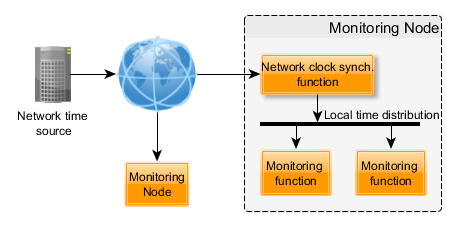
\includegraphics[width=0.45\textwidth]{figures_raw/concept.png}
    \caption{Conceptual model of distributed monitoring framework}
    \label{fig:concept}
\end{figure}

As seen on Figure~\ref{fig:concept} each node has it's own network synchronization function therefore the accuracy and
precision between two monitoring nodes can be guaranteed only to an extent that the utilized time synchronization
protocol provides. This is in the magnitude of milliseconds of a software implementation of NTP -- however with FPGA
based implementation
this precision can be increased --  and in the magnitude of
microseconds or nanoseconds depending on the PTP version used and also on the underlying network.
The key concept is that over the local time distribution bus even greater synchronicity can be achieved as there is
less
perturbation between the HW implementations of the transmitting and receiving ends -- no OS scheduler, no network
\emph{etc.} --
and also frequency synchronization can be easily achieved by implementing a synchronous bus -- \emph{i.e.} transmitting
the
clock signal along with the data.

\subsection{External time synch. subsystem design and implementation}\label{sec:External-Impl}

When selecting the candidate for implementing the external time synchronization function
three protocols were considered:
\begin{itemize}
    \item Network Time Protocol
    \item Precision Time Protocol v1
    \item Precision Time Protocol v2
\end{itemize}

In order to achieve the best synchronization between PTPv2 clocks the protocol requires PTPv2 enabled switches/routers
in the network for bookkeeping the processing delay values in the synchronization packets as they traverse through the
network.
In a multi-hop network without having that feature the achievable synchronicity is around the same that can be reached
using
PTPv1.
That concluded in either selecting NTP or PTPv1. Nevertheless PTPv1 has way more mode of operation compared to NTP but
when comparing these two protocols they are semantically operating based on the same principle to determine the round
trip time and offset
compared to a reference clock entity. However there are significant differences coming from the packet structure, the
timestamp format and the nomenclature that could result in slower implementation had the latter protocol been chosen.
While in NTP the timestamp format is ... TODO(fecjanky): compare  NTP and PTP timestamps
The design decision based on the considerations above led to selecting NTP protocol to be used for synchronizing the
FPGA based monitoring cards through a card that is responsible for implementing the external and internal (see
Section!\ref{sec:Internal-Impl}) time synchronized function called SGA-Clock.

FPGA based packet processing and networking protocol implementations have their own complexity. There are several
readily available implementations that can be used for packet processing in FPGAs with more or less flexibility when it
comes to interconnecting it
with other modules. The one that has been used for the implementation is a flexible solution for  Protocol
Implementations within FPGAs detailed in \cite{ProtoImpl} which provides a generic framework in VHSIC Hardware
Description Language (VHDL) that enables rapid prototyping of networking protocols. Among many other things it provides
the following main features
\begin{itemize}
    \renewcommand \labelitemi{--}
    \item supports protocol module interconnection via layering;
    \item handles reception and transmission of PDUs with queuing;
    \item provides a high level interface for separating and combining	Protocol Control Information (PCI) and SDU,
          forwarding, pausing or dropping SDUs;
    \item provides a unified way to handle ICI, SDU, and PDU events (e.g error signalling);
    \item adds support of auxiliary information that travels along with messages
    \item provides components for common tasks recurring during implementing networking protocols
          (de/serialization, arbitration etc.).
\end{itemize}

\begin{figure}[!htb]
    \centering
    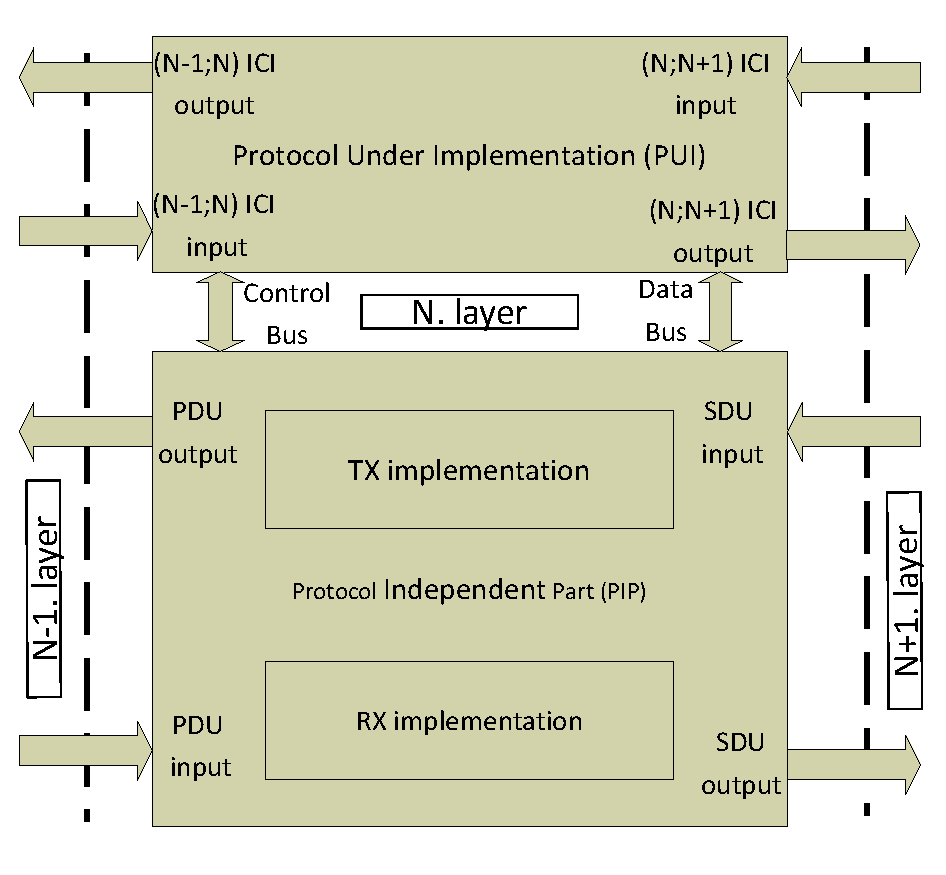
\includegraphics[width=0.4\textwidth]{figures_raw/system_sketch.pdf}
    \caption{Fundamental building block of the FPGA networking framework used for the protocol stack implementation}
    \label{fig:system_sketch}
\end{figure}

The framework's basic building block (shown on Figure~\ref{fig:system_sketch}) was used for implementing pure FPGA
hardware based
UDP/IP protocol stack with ARP on top of 802.3 Ethernet that provides a platform with deterministic timing for the
likewise FPGA based
implementation of NTP. For each of these protocols the corresponding protocol specific parts have been described in
VHDL using the generic framework.

\begin{figure}[!htb]
    \centering
    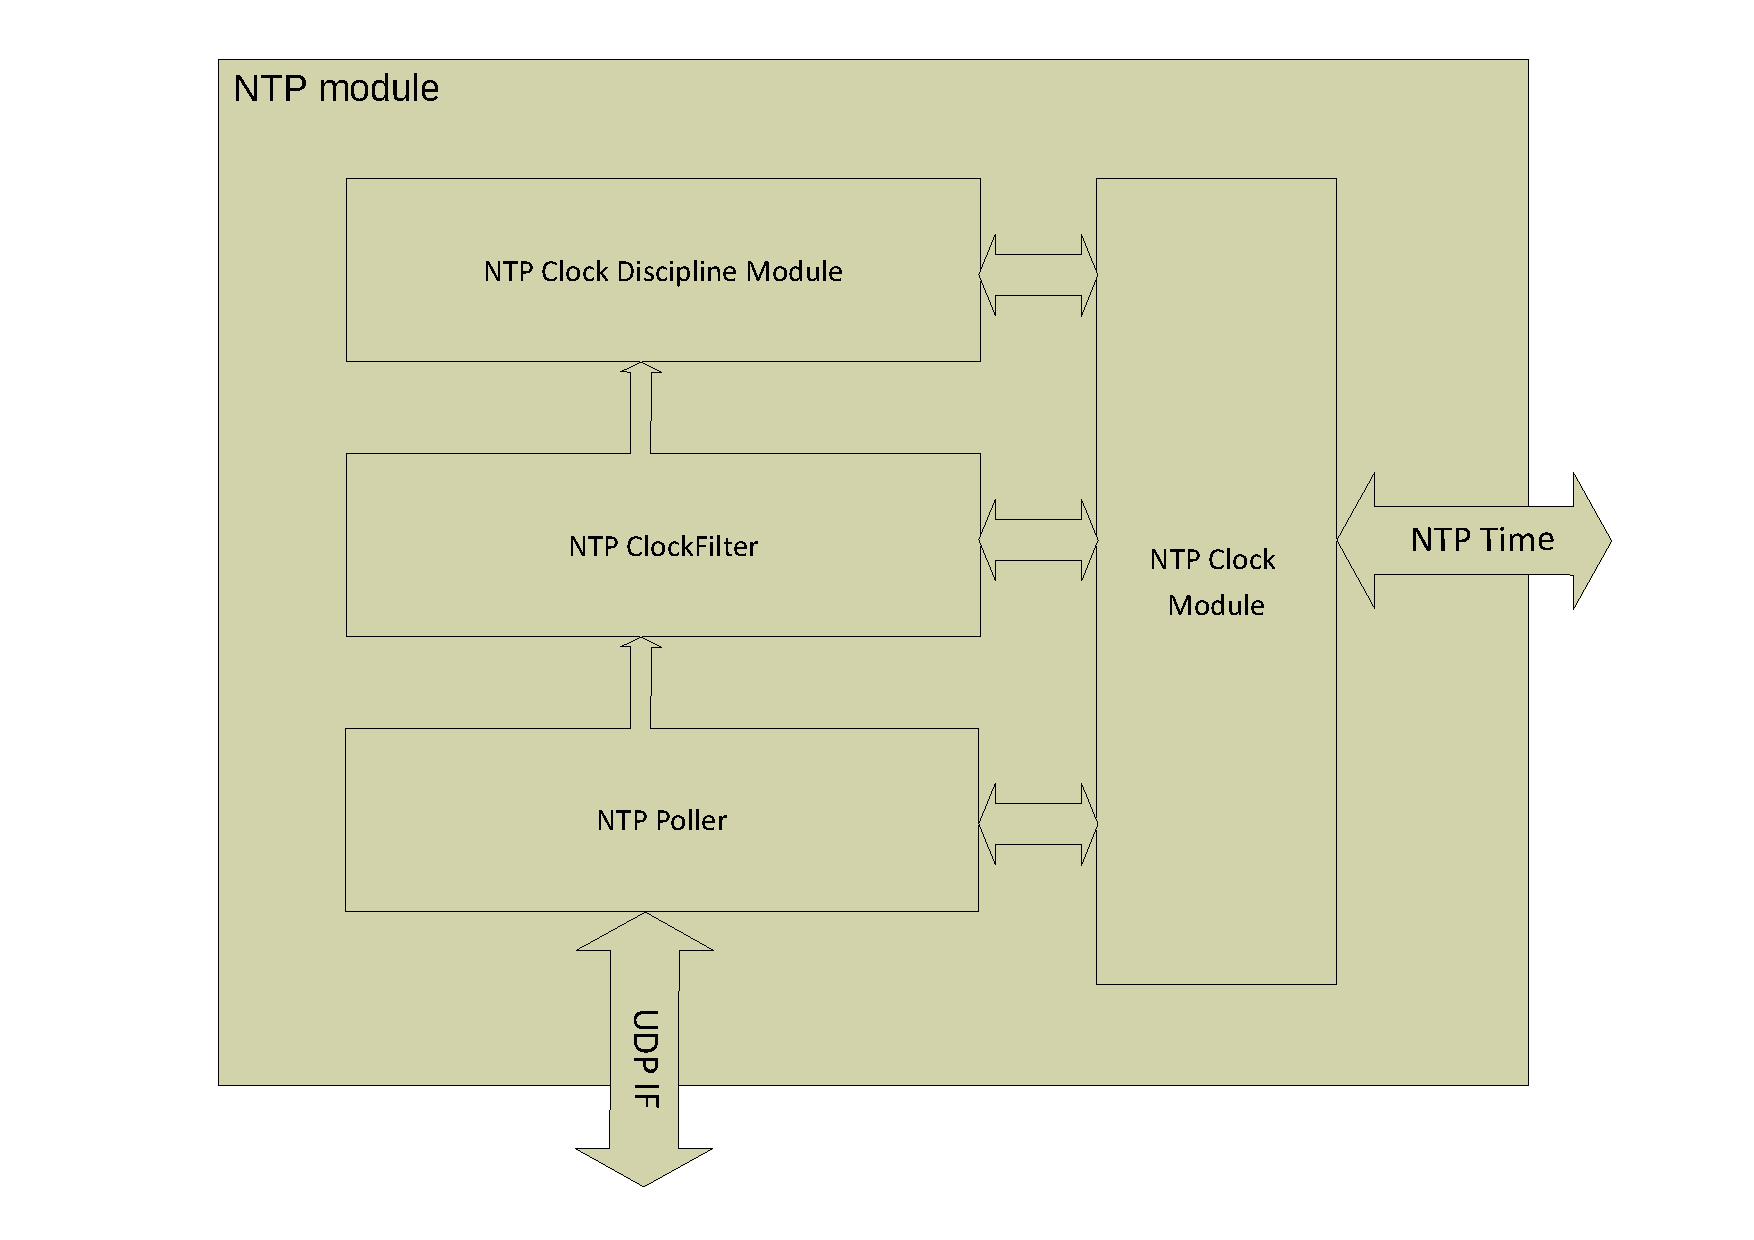
\includegraphics[width=0.5\textwidth]{figures_raw/ntp-sketch.pdf}
    \caption{NTP module block diagram of components}
    \label{fig:ntp-impl}
\end{figure}

The internal structure of the NTP module is shown on Figure~\ref{fig:ntp-impl}. The NTP Poller component is responsible
for the NTP packet transmission and reception and implementing the On-Wire protocol
for determining the offset  -- based on the packet messages. The network packet handling part is also implemented
through the Protocol Implementations framework. The NTP ClockFilter component is there to regulate the offset values
presented by the poller by ordering the results based on delay, updating internal state variables, calculating jitter,
and
suppressing spikes based on jitter and last successful test time. If the offset data passed the filter stage it is
forwarded for further processing by the discipline module.

The NTP Discipline module controls the clock module -- by adjusting the time increment -- based on the filtered offset
data. The NTP clock module provides an interface for controlling the time increment that itself is added to the clock
register in each system clock cycle thus
implementing the clock functionality. The time information is fed back to each module as illustrated on
Figure~\ref{fig:ntp-impl}.
This chain of modules with the feedback is another realization of a closed loop control chain as described in
Section~\ref{sec:Internal-Impl}.

\subsection{Internal time synch. subsystem design and implementation}\label{sec:Internal-Impl}

The internal time information synchronization function is responsible for having all clocks in all monitoring functions
to be completely synchronized within a monitoring node. Since this is an internal component the amount of perturbation
that potentially affects this subsystem is considered minimal compared to the external time synchronization subsystem.

The elements of this subsystem are:
\begin{itemize}
    \item digital bus that is able to transmit time and status information
    \item a driver module of that bus that resides in the Network clock synchronization function
    \item receiver modules attached to that bus performing local time synchronization
\end{itemize}

Internally all FPGA boards implementing a monitoring function can operate from different power supply units as a
consequence ground level
isolation is necessary over the bus. For reducing the physical layer complexity
a point-to-point bus system has been designed. To be able to maximize the number of connected clients connected the
bus utilizes an asynchronous serial communication using 2 wires. The communication protocol executed by the driver
module
multiplexes arbitrary data units and the time information over the bus into frames -- equipped with error detection
code --
in an alternating pattern.That results in periodic transmission of valid time information.

The parameters of the physical signalling are:
\begin{itemize}
    \item LVCMOS33 levels for representing logical values
    \item asymmetric signal transmission
    \item \SI{15.625}{\mega\hertz} clock frequency with 4x oversampling
    \item NRZ coding
\end{itemize}

The frame format used on the bus is shown on Figure~\ref{fig:HiSTI-frame}. The frame starts with an all 1's preamble
followed by a start bit with value 0. The type field is used to discriminate between the payload type, when T=1 it
indicates that the payload is
time information otherwise it's data -- on this data channel an overlay data communication protocol can be used.
The time format is in line with the external time synchronization \emph{i.e.} it uses the NTP
time format for representing the time information. For detecting transmission errors on the bus a CRC-8 value is
calculated
for the \emph{`Type'} and \emph{`Payload'} fields and appended to the frame that is checked on frame reception for
detecting
transmission errors.

Given the parameters above the frame time is 90/\SI{15.625}{\mega\hertz} = \SI{5.76}{\micro\second} and since every
other frame carries time information the clock on the receiver side can be disciplined/controlled on a
\SI{11.52}{\micro\second}
basis. Under such short period of time even low quality, non-temperature controlled crystal oscillators have negligible
drift
as a result this update period is adequate for the network monitoring use case.

\begin{figure}
    \begin{bytefield}{32}
        \bitheader{0-31} \\
        \bitbox{16}{All ones} & \bitbox{1}{S} & \bitbox{1}{T} & \bitbox{14}{time/data} \\
        & \wordbox{1}{time/data} \\
        & \bitbox{18}{} & \bitbox{8}{CRC-8}
    \end{bytefield}
    \caption{High-Speed Timestamp Interface frame format}
    \label{fig:HiSTI-frame}
\end{figure}

The receiver module de-multiplexes the data and the time information from the payload of the received frame. It also
verifies that the received frame's CRC-8 value matches the calculated one. If no errors were detected then it feeds the

time information into a module that performs time synchronization using a closed loop control.
This closed loop control has a simple proportional controller as illustrated on Figure~\ref{fig:closed-loop}. The clock
module
is incrementing a clock counter with an increment in each system clock period. Since the oscillator frequency was not
configurable in
existing system the way to discipline the clock was through adjusting the time increment itself.
Even though the increment is adjusted proportionally to the error signal it is a integral controller due to nature of
the time increment process that adds the current time increment to the time counter on each clock cycle
-- \emph{i.e.} integral of a function of the error signal over time.

\begin{figure}[H]
    \centering
    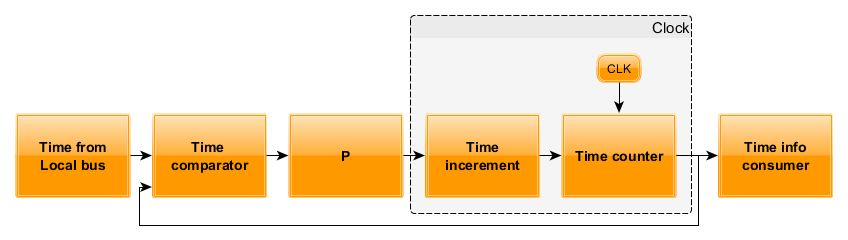
\includegraphics[width=0.45\textwidth]{figures_raw/time_control_loop.png}
    \caption{Internal clock control loop}
    \label{fig:closed-loop}
\end{figure}

In theory a I controller in a closed loop system can eliminate error signal -- \emph{i.e.} the time difference --
completely.
With this design the solution contains a digital time distribution bus and a module that realizes the
closed control loop as seen on Figure~\ref{fig:closed-loop}.

\subsection{Realized system}

The realized system with all internal components is shown on Figure~\ref{fig:realized-system} where the external time
synchronization -- as presented in Section~\ref{sec:External-Impl} -- is done by the SGA Clock card -- visible in the
bottom right part -- and the internal time synchronization -- described in Section~\ref{sec:Internal-Impl} --
is performed over the local bus with agent modules synthesized in all monitoring cards acting as slaves on the
high-speed timestamp interfaces also driven by the SGA Clock card acting as a master.

\begin{figure}[H]
    \centering
    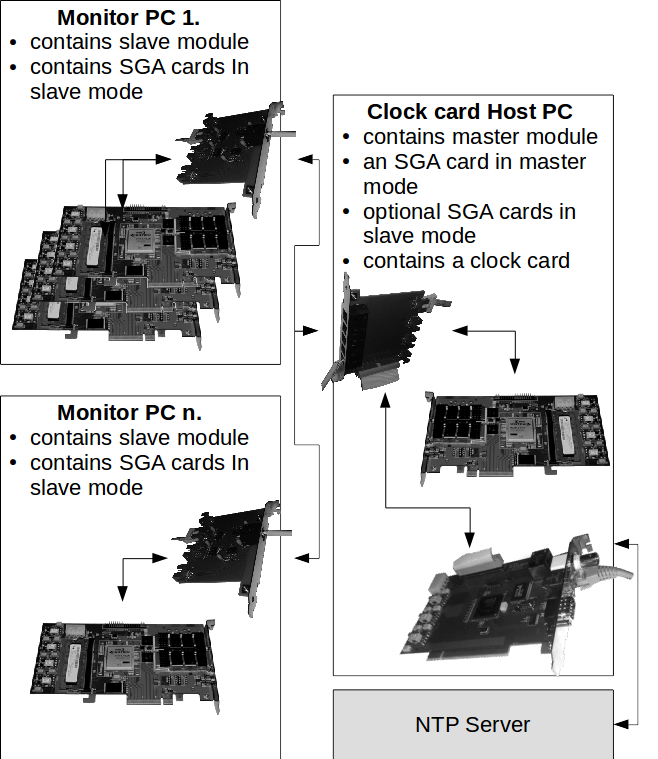
\includegraphics[width=0.45\textwidth]{figures_raw/clock_architecture.png}
    \caption{The realized system with all internal components}
    \label{fig:realized-system}
\end{figure}

\section{Verification \& Results}

%TODO(Fec) : 1.5 oldal
%- Describe the verification method in detail
%- Matlab graph, long-term vs. short-term 

For verifying the solution extensive testing and measurements have been carried out. For inspecting the degree of
synchronization to the master NTP clock a packet capturer operating in promiscuous mode was installed on the Ethernet
segment on which the FPGA implementation of the NTP slave was connected. The NTP packets used for synchronization were
captured bidirectionally. This packet capture then was filtered for those NTP packets that had all 4 timestamps used in

the On-Wire protocol to calculate the offset from the reference clock value. With software based post-processing the
offset information was extracted along with the time elapsed from the start of measurement -- which is determined by
the
first NTP packet present in the packet capture.

\begin{figure*}[!htb]
    \centering
    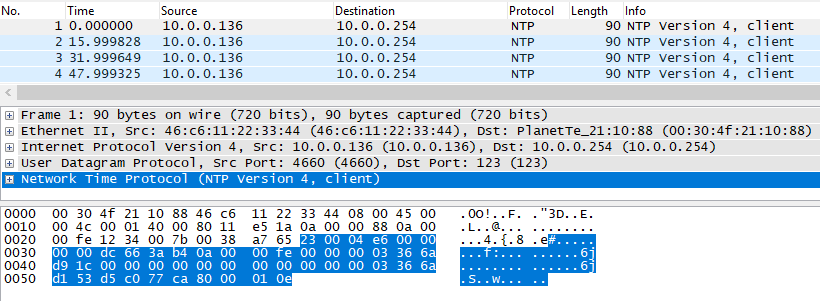
\includegraphics[width=0.9\textwidth]{figures_raw/pcap-NTP.png}
    \caption{Measurement results - packet capture}
    \label{fig:pcap-NTP}
\end{figure*}

A sample packet capture is visible on Figure~\ref{fig:pcap-NTP}. The statistical parameters -- like the drift and real
offset -- of the device was determined by
fitting a linear curve on the offset values. For the actual measurement presented in this paper the capture was taken
for approximately 3 hours.
The measurement values and the fitted curve plot can be seen on Figure~\ref{fig:results}.

\begin{figure*}[!htb]
    \centering
    \includegraphics[width=0.9\textwidth]{figures_raw/plot2.png}
    \caption{Measurement results - plot of derived data}
    \label{fig:results}
\end{figure*}

The curve fitted on this measurement shows that there was a fix \SI{14.52}{\micro\second} offset compared to the
reference clock. As presented in Section~\ref{sec:Challanges}
having a precise and stable clock -- with known offset -- is as good as having an accurate one. As for the stability
the first order stability of the
device is \SI{-0.7}{1/\nano\second}. This precision and stability are considered adequate for satisfying the
requirements of the external time synchronization part.

As for the internal synchronization part it is by design accurate as it is a synchronous bus system with no
disturbances -- under normal operating conditions -- as a
consequence the clock accuracy over that bus is determined by the bit width and the refresh rate of the digital
time-stamp transmitted over the bus. As it was described in Section~\ref{sec:Internal-Impl} the
time-stamp is 64 bits wide also using the NTP binary fractional representation. Given that the time-stamp is accurate
to the last bit then the theoretical accuracy is \SI{232.83}{\pico\second}.

\section{Conclusion}

TODO(Fec \& Pali): 0.5 oldal

References: 0.5 oldal

% http://www.ctan.org/tex-archive/biblio/bibtex/contrib/doc/
% The IEEEtran BibTeX style support page is at:
% http://www.michaelshell.org/tex/ieeetran/bibtex/

%\bibliographystyle{IEEEtran}
% argument is your BibTeX string definitions and bibliography database(s)
%\bibliography{references}

%
% <OR> manually copy in the resultant .bbl file
% set second argument of \begin to the number of references
% (used to reserve space for the reference number labels box)

%\begin{thebibliography}{1}
%
%\bibitem{IEEEhowto:kopka}
%H.~Kopka and P.~W. Daly, \emph{A Guide to \LaTeX}, 3rd~ed.\hskip 1em plus
% 0.5em minus 0.4em\relax Harlow, England: Addison-Wesley, 1999.
%
% \end{thebibliography}

\end{document}
